\chapter{Hình học của vũ trụ giãn nở}

Trọng tâm ở đây là vũ trụ giãn nở và hình học của nó. Mục đích là mô tả không gian giãn nở có nghĩa là gì trước khi hỏi điều gì chi phối sự giãn nở ấy. Phần vũ trụ học Newton với \(F=ma\) sẽ đến sau, và chỉ sau đó hình học và động lực học mới được ghép lại thành khuôn khổ Friedmann--Robertson--Walker đầy đủ.

\section{Tọa độ đồng chuyển trên một đường thẳng giãn nở}

Hãy bắt đầu với ví dụ đơn giản nhất có thể: không gian một chiều, không phải không-thời gian. Hãy hình dung một đường thẳng vô hạn với các thiên hà cách đều nhau trên đó. Tọa độ \(x\) chưa đo một khoảng cách vật lý. Nó dùng để gán nhãn các thiên hà. Có thể xem \(x\) như tên của một thiên hà, và cái tên ấy vẫn gắn với thiên hà đó ngay cả khi toàn bộ cấu hình bị kéo giãn hoặc co lại.

Gọi khoảng cách vật lý từ thiên hà mang tên \(x=0\) đến thiên hà mang tên \(x=1\) là \(a\). Khi đó khoảng cách vật lý giữa bất kỳ hai thiên hà nào là
\begin{equation}
d=a\,\Delta x.
\end{equation}
Độ chênh tọa độ \(\Delta x\) chỉ đơn thuần là hiệu giữa các nhãn. Thừa số \(a\) biến hiệu nhãn đó thành một khoảng cách thực sự được đo bằng thước mét.

Bây giờ hãy hình dung đường thẳng như một sợi dây đàn hồi đang bị kéo giãn. Các nhãn vẫn đi cùng các thiên hà, nhưng khoảng cách giữa các thiên hà lân cận thay đổi theo thời gian. Hệ thức đó trở thành
\begin{equation}
d(t)=a(t)\,\Delta x.
\end{equation}
Ở giai đoạn này, tính đồng nhất đơn giản chỉ có nghĩa là các thiên hà lân cận cách đều nhau ở mọi nơi, mặc dù khoảng cách chung ấy có thể biến thiên theo thời gian.

\section{Định luật Hubble và việc không có tâm}

Để tìm vận tốc tương đối của hai thiên hà cố định, hãy giữ cặp ấy cố định sao cho \(\Delta x\) không đổi theo thời gian. Lấy đạo hàm ta được
\begin{align}
\dot d &= \dot a\,\Delta x \\
       &= \frac{\dot a}{a}\,a\,\Delta x \\
       &= \frac{\dot a}{a}\,d.
\end{align}
Nếu ta định nghĩa
\begin{equation}
H(t)\equiv \frac{\dot a}{a},
\end{equation}
thì
\begin{equation}
\dot d = H(t)\,d.
\end{equation}
Đây là định luật Hubble.

Cụm từ lịch sử ``hằng số Hubble'' dễ gây hiểu lầm. Đại lượng này là hằng theo không gian, không phải theo thời gian. Tại một thời điểm cho trước, nó là như nhau đối với mọi thiên hà, nhưng nói chung nó thay đổi khi vũ trụ tiến hóa. Tốt hơn nên xem nó là tham số Hubble.

Định luật nói rằng các thiên hà ở xa hơn lùi ra xa nhanh hơn. Nó không chọn ra một tâm nào. Không có gì trong lập luận ưu tiên \(x=0\), hay bất kỳ điểm nào khác. Mọi quan sát viên đều thấy cùng một quy luật. Vì thế, trong mô hình này, vũ trụ giãn nở không phải là một vụ nổ từ một vị trí đặc biệt nào đó.

Dịch đỏ xuất hiện ngay lập tức. Nếu hai thiên hà trao đổi tín hiệu ánh sáng trong khi đang tách xa nhau, ánh sáng nhận được bị dịch đỏ. Vận tốc lùi càng lớn thì độ dịch đỏ càng lớn. Vì vậy, các vạch phổ cho ta biết về các vận tốc lùi. Khoảng cách thì khó đo hơn, và các ước lượng ban đầu của Hubble khá thô. Đồ thị đầu tiên của ông không phải là một đường thẳng hoàn hảo mà là một tập hợp điểm phân tán với độ bất định lớn. Dẫu vậy, nguyên lý hình học vẫn vượt qua được nhiễu: vận tốc lùi tỉ lệ với khoảng cách.

\begin{classroomqa}
\audiencequestion{Nếu các thiên hà ở đủ xa nhau, thì định luật Hubble có khiến chúng chuyển động nhanh hơn tốc độ ánh sáng không?}\lecturetimestamp{00:20:23}
\lecturerresponse{Có, theo nghĩa lùi xa này thì có. Điều bạn nói là đúng. Chúng ta chắc chắn sẽ quay lại điểm đó. Đó là một trong những điều quan trọng nhất.}
\end{classroomqa}

\section{Số chiều cao hơn, tính đẳng hướng và sự phụ thuộc theo thời gian của \(a(t)\)}

Không có gì cốt yếu thay đổi khi thêm nhiều chiều không gian hơn. Trong hai chiều, hãy hình dung một mạng lưới vuông các thiên hà được gắn nhãn bằng \((x,y)\), và trong ba chiều bằng \((x,y,z)\). Các tọa độ một lần nữa là những nhãn đồng chuyển. Chúng đi cùng các thiên hà thay vì trực tiếp đo khoảng cách vật lý.

Vì sao khoảng cách theo hướng \(x\) lại phải giống khoảng cách theo hướng \(y\)? Câu trả lời đến từ quan sát. Nếu các thiên hà có hệ thống tập trung dày hơn theo một hướng so với hướng khác, thì bầu trời sẽ trông khác nhau theo các hướng khác nhau. Trên các thang đủ lớn thì không như vậy. Sự giống nhau theo hướng ấy là tính đẳng hướng.

Trong hai chiều, khoảng cách giữa hai thiên hà là
\begin{equation}
d=a\sqrt{(\Delta x)^2+(\Delta y)^2},
\end{equation}
và trong ba chiều là
\begin{equation}
d=a\sqrt{(\Delta x)^2+(\Delta y)^2+(\Delta z)^2}.
\end{equation}
Đối với một cặp thiên hà cố định, các độ chênh tọa độ giữ nguyên, nên lấy đạo hàm một lần nữa cho
\begin{equation}
\dot d=\frac{\dot a}{a}\,d.
\end{equation}
Định luật Hubble không thay đổi.

Tính đồng nhất nghĩa là sự giống nhau từ nơi này sang nơi khác. Tính đẳng hướng nghĩa là sự giống nhau từ hướng này sang hướng khác. Cả hai đều không chính xác trên các thang nhỏ. Nhìn xuyên qua Ngân Hà khác với nhìn ra khỏi mặt phẳng của nó, và các thiên hà riêng lẻ không phân bố đồng đều ở các khoảng cách ngắn. Nhưng sau khi lấy trung bình trên nhiều thiên hà, vũ trụ ở thang lớn trông xấp xỉ như nhau ở mọi nơi và theo mọi hướng.

\begin{classroomqa}
\audiencequestion{Nếu vận tốc tỉ lệ với khoảng cách, và khoảng cách đang tăng lên, điều đó có nghĩa là một cặp thiên hà cố định phải đang tăng tốc rời xa nhau không?}\lecturetimestamp{00:40:22}
\lecturerresponse{Không. Định luật Hubble nói rằng tại một thời điểm cho trước, vận tốc lùi tỉ lệ với khoảng cách. Tự nó không nói liệu vận tốc của một cặp cố định tăng hay giảm theo thời gian. Điều đó phụ thuộc vào sự phụ thuộc theo thời gian chi tiết của \(a(t)\). Nếu \(a(t)\propto t\), các thiên hà lân cận tách ra với vận tốc không đổi. Nếu \(a(t)\propto t^2\), vận tốc lùi của một cặp cố định tăng theo thời gian. Nếu \(a(t)\propto \log t\), nó giảm theo thời gian. Định luật \(\dot d=(\dot a/a)d\) luôn đúng như một hàm của khoảng cách, nhưng tăng tốc và giảm tốc là những câu hỏi riêng biệt.}
\end{classroomqa}

Trong một thời gian dài, các nhà vũ trụ học đã kỳ vọng vũ trụ đang giảm tốc, vì lực hấp dẫn lẽ ra phải làm chậm một sự giãn nở ban đầu giống như cách lực hấp dẫn làm chậm một vật bị ném lên trên. Ở đây, điểm cần nhấn mạnh chỉ là bản thân định luật Hubble không quyết định được hành vi của \(\dot a\) hay \(\ddot a\).

\begin{classroomqa}
\audiencequestion{Làm thế nào để đặt giá trị ban đầu của thừa số tỉ lệ \(a\)?}\lecturetimestamp{00:46:18}
\lecturerresponse{Chuẩn hóa tổng thể của nó là tùy ý. Điều quan trọng về mặt vật lý không phải là độ lớn bằng số của \(a\) tự nó, mà là nó thay đổi như thế nào. Nếu ta định nghĩa một thừa số tỉ lệ khác \(b=3a\), thì \(\dot b/b=\dot a/a\). Việc đổi chuẩn \(a\) bằng một hằng số làm thay đổi quy ước hoặc đơn vị, chứ không làm thay đổi tham số Hubble.}
\end{classroomqa}

\section{Từ mêtric không gian đến mêtric không-thời gian}

Bây giờ thay \(\Delta x\) bằng \(dx\). Khoảng cách vật lý giữa các điểm lân cận là
\begin{equation}
ds=a\,dx,
\end{equation}
nên
\begin{equation}
ds^2=a^2\,dx^2.
\end{equation}
Đây là mêtric không gian trong một chiều. Hệ số của \(dx^2\) là
\begin{equation}
g_{xx}=a^2.
\end{equation}
Vì thế, có thể mô tả một vũ trụ giãn nở bằng cách nói rằng phần không gian của mêtric phụ thuộc vào thời gian.

Để chuyển từ không gian sang không-thời gian, dùng khoảng tương đối tính. Trong một chiều không gian,
\begin{equation}
d\tau^2=dt^2-a^2(t)\,dx^2.
\end{equation}
Đối với một quan sát viên đồng chuyển, \(dx=0\), nên \(d\tau=dt\). Thời gian vũ trụ thông thường là thời gian riêng được đo bởi các đồng hồ chuyển động cùng các thiên hà.

Hình vẽ trên bảng ở chỗ này rất hữu ích vì nó đặt các đường thế giới đồng chuyển, phần tử độ dài và ký hiệu mêtric lại với nhau.
\begin{figure}[H]
\centering
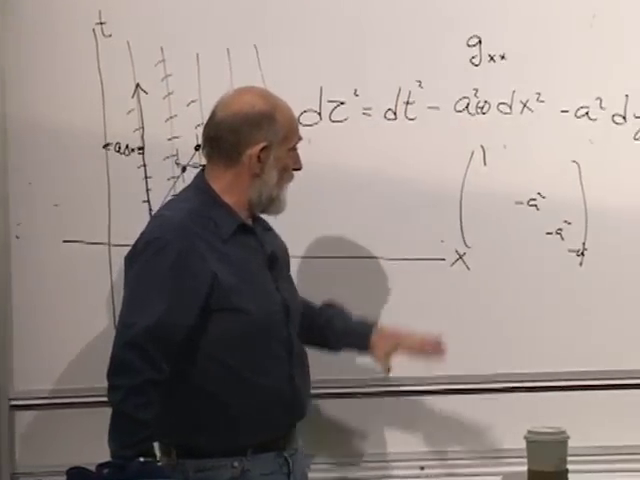
\includegraphics[width=0.82\textwidth]{lecture_01_figure_02.png}
\caption{Các đường thế giới đồng chuyển trong một vũ trụ một chiều giãn nở cùng với khoảng không-thời gian tương ứng.}
\end{figure}

Trong ba chiều không gian, cùng một mẫu cho phép mở rộng thận trọng sau đây\footnote{Phần bảng quanh 00:56:38--00:58:51 bị che khuất một phần. Dạng ba chiều này được suy ra từ phần mở rộng bằng lời từ một chiều không gian lên ba chiều, cùng với mẫu đường chéo nhìn thấy trên bảng.}
\begin{equation}
d\tau^2=dt^2-a^2(t)\bigl(dx^2+dy^2+dz^2\bigr),
\end{equation}
với mêtric đường chéo
\begin{equation}
g_{\mu\nu}=\mathrm{diag}\bigl(1,-a^2,-a^2,-a^2\bigr).
\end{equation}
Các phần tử ngoài đường chéo triệt tiêu,
\begin{equation}
g_{tx}=g_{ty}=g_{tz}=0.
\end{equation}

Tính đồng nhất nghĩa là các hệ số mêtric có thể phụ thuộc vào thời gian nhưng không phụ thuộc vào vị trí không gian. Tính đẳng hướng nghĩa là ba hướng không gian xuất hiện theo cùng một cách.

\begin{classroomqa}
\audiencequestion{Chẳng phải ta nên xem \(dx\) là một khoảng cách sao?}\lecturetimestamp{01:01:18}
\lecturerresponse{Không. \(dx\) không phải là khoảng cách. \(a\,dx\) mới là khoảng cách. \(dx\) chỉ đơn thuần là một khoảng chênh giữa các nhãn. Một cách hữu ích để nghĩ về nó là hãy hình dung rằng, tại một thời điểm nào đó, có người vẽ một lưới tọa độ xuyên qua các thiên hà rồi buộc lưới ấy đi theo chúng. Độ tách tọa độ được giữ cố định theo cách xây dựng, còn khoảng cách vật lý thì thay đổi. Ta có thể đưa đơn vị độ dài vào \(x\) thay vì vào \(a\); đó là một quy ước. Điều quan trọng là tích \(a\,dx\).}
\end{classroomqa}

\begin{classroomqa}
\audiencequestion{Hệ số mêtric của \(dt^2\) bằng \(1\). Điều đó cũng chỉ là do quy ước thôi sao?}\lecturetimestamp{01:03:24}
\lecturerresponse{Đúng vậy. Tự bản thân điều đó không mang nội dung vật lý nào. Nếu hệ số ấy chỉ phụ thuộc vào thời gian, ta có thể đổi biến thời gian để nó trở thành đơn giản là \(dt^2\). Tương tự, ta có thể chọn đơn vị với \(c=1\). Điều không phải là quy ước ở đây là hệ số ấy không phụ thuộc vào vị trí, mặc dù nó có thể phụ thuộc vào thời gian.}
\end{classroomqa}

\begin{classroomqa}
\audiencequestion{Nếu đưa điều này vào các phương trình trường Einstein, thì ta sẽ thu được gì cho tensor năng lượng-động lượng?}\lecturetimestamp{01:05:59}
\lecturerresponse{Đó là dạng câu hỏi kế tiếp, nhưng nó thuộc về động lực học chứ không thuộc cuộc thảo luận hiện tại. Người ta có thể đưa metric này vào các phương trình Einstein và hỏi phân bố năng lượng-động lượng nào sẽ khiến nó trở thành một nghiệm. Điều đó rất quan trọng, nhưng lúc này chủ đề là hình học, không phải động lực học.}
\end{classroomqa}

\section{Những gì chân trời che khuất}

Vũ trụ ở quy mô lớn chỉ được xem là đồng nhất và đẳng hướng như một phép gần đúng. Chắc chắn nó không đồng nhất ở thang của các ngôi sao, các hành tinh, hay thậm chí của từng thiên hà riêng lẻ. Nó cũng không hoàn toàn đẳng hướng trong mọi quan sát cục bộ.

Một cánh đồng của người nông dân minh họa đúng sự phụ thuộc vào thang. Ở một thang, nó trông đều đặn; ở một thang nhỏ hơn nhiều, rõ ràng là không; còn ở một thang lớn hơn cả cánh đồng, nó lại không còn trông đồng nhất nữa. Vũ trụ học cũng vận hành theo cách như vậy. Sau khi lấy trung bình trên nhiều thiên hà, phân bố ở quy mô lớn trông gần như đồng đều. Ở những thang đủ nhỏ thì không như vậy.

Vũ trụ lớn hơn phần mà ta có thể thấy, và lớn hơn cả phần mà ta có thể thấy được vào bất kỳ lúc nào. Ở những thang thực sự có thể khảo sát được, nó là đẳng hướng và đồng nhất, ngoại trừ các biến thiên cục bộ. Vượt ra ngoài đó thì không có bảo đảm trực tiếp nào từ quan sát.

\begin{classroomqa}
\audiencequestion{Ông nói rằng rốt cuộc chúng ta sẽ không bao giờ trực tiếp tìm ra được. Điều đó có ngụ ý rằng có thể có một cách gián tiếp để tìm ra không?}\lecturetimestamp{01:10:34}
\lecturerresponse{Có lẽ. Phần lớn cách nghĩ ngày nay là ở những thang đủ lớn thì vũ trụ không đồng nhất, và tôi cũng nghiêng về phía đó. Nhưng đó là một canh cược mà tôi sẽ không bao giờ thắng cũng không bao giờ thua, bởi vì do những lý do cơ bản mang tính nền tảng, chúng ta sẽ không thể nhìn xa hơn nhiều so với những gì có thể thấy bây giờ. Đó là sự tồn tại của một chân trời.}
\end{classroomqa}

\begin{classroomqa}
\audiencequestion{Chẳng lẽ không thể dùng hấp dẫn để tìm các khối lượng nằm ngoài phần ta có thể nhìn thấy sao?}\lecturetimestamp{01:11:53}
\lecturerresponse{Không. Một khối lượng ở xa có thể đơn giản chỉ khiến ta rơi tự do. Ngồi trong một căn phòng kín, ta ở trong trường hấp dẫn của Mặt Trời và quay quanh nó, nhưng nếu không nhìn ra ngoài thì không có cách dễ dàng nào để biết rằng Mặt Trời ở đó. Chỉ có các lực thủy triều mới bộc lộ điều đó, và nếu nguồn ở đủ xa thì các hiệu ứng thủy triều ấy có thể quá nhỏ để phát hiện.}
\end{classroomqa}

Vì thế, chân trời là một rào cản tối hậu đối với tri thức trực tiếp. Ông thậm chí còn nói, gần như chắc chắn, rằng vũ trụ có thể tích ít nhất lớn hơn một nghìn lần so với vùng mà ta có thể thấy được, dù có đợi bao lâu đi nữa, và để phần giải thích cho nhận định ấy đến sau.

\section{Hữu hạn mà không có biên}

Bây giờ chuyển sang các hình học đóng. Đường thẳng vô hạn là mở và không bị chặn. Một đoạn thẳng là bị chặn theo nghĩa chỉ có một phạm vi hữu hạn. Bị chặn không có nghĩa là có biên, mà là có phạm vi hữu hạn.

Một khối lập phương có tường thì không được. Nó vi phạm tính đồng nhất, vì người ở gần một bức tường không tương đương với người ở xa tường, và nó vi phạm tính đẳng hướng, vì ngay cả người ở tâm cũng thấy những thứ khác nhau theo các hướng khác nhau.

Phần bên trong của một hình tròn hay một khối cầu cũng không đạt. Người ở tâm thấy cùng một thứ theo mọi hướng, nhưng tính đối xứng đó chỉ thuộc về một điểm đặc biệt duy nhất. Rời khỏi tâm thì bức tường ở gần theo một hướng và ở xa theo hướng khác. Khi đó không gian vừa không đồng nhất vừa không đẳng hướng đối với các quan sát viên điển hình.

Ở những quy mô rất lớn, giả định làm việc là vũ trụ đồng nhất và đẳng hướng. Đó là nguyên lý vũ trụ học. Nó hữu ích, nhưng không được miễn khỏi khả năng phải xét lại.

\begin{classroomqa}
\audiencequestion{Tính đẳng hướng ở mọi nơi có kéo theo tính đồng nhất không?}\lecturetimestamp{01:18:57}
\lecturerresponse{Có. Nếu mọi quan sát viên đều thấy cùng một cảnh tượng theo mọi hướng, thì điều đó kéo theo tính đồng nhất. Nhưng mệnh đề đảo là sai. Bản thân tính đồng nhất không kéo theo tính đẳng hướng. Một vũ trụ có thể đồng nhất mà vẫn có một hướng ưu tiên, chẳng hạn nếu nó được lấp đầy bằng những mũi tên cùng chỉ theo một hướng.}
\end{classroomqa}

Mô hình hữu hạn đúng là bề mặt của một hình cầu không có đặc điểm phân biệt nào. Một sinh vật hai chiều bị giới hạn trên bề mặt ấy sẽ thấy mọi nơi, xét cục bộ, đều giống mọi nơi khác và mọi hướng đều giống mọi hướng khác, dù thế giới là hữu hạn. Đó là hữu hạn mà không có biên.

\section{Một vũ trụ một chiều đóng trên một đường tròn}

Để giữ cho đại số đơn giản, hãy rút ví dụ về hình cầu xuống còn một chiều không gian: sự sống trên một đường tròn. Trong một chiều, tính đẳng hướng có nghĩa là trái và phải là tương đương. Một đường tròn có đúng đặc điểm đó. Chọn một điểm và gọi nó là \(\theta=0\). Mọi điểm khác được gán bởi một tọa độ góc \(\theta\), đo bằng radian. Một điểm nằm ngay về một phía của gốc có thể được mô tả hoặc bằng một góc âm nhỏ, hoặc bằng một góc chỉ kém \(2\pi\) một chút. Tính tuần hoàn đó là một phần của hình học.

Cư dân trên đường tròn tiếp cận được chu vi, chứ không tiếp cận được một bán kính hay một tâm từ bên ngoài. Họ có thể đo tổng quãng đường quanh vòng bằng cách đi dọc theo đường tròn cho đến khi quay trở lại đúng điểm cũ. Nếu vẽ đường tròn trong một mặt phẳng ngoại tại, ta cũng có thể đưa vào một đại lượng kiểu bán kính, nhưng đại lượng đó thuộc về bức tranh nhúng, không thuộc hình học nội tại mà họ đo được.

Hình vẽ trên bảng ở đây rất hữu ích vì nó giữ các nhãn góc và tổng chu vi trong cùng một hình.
\begin{figure}[H]
\centering
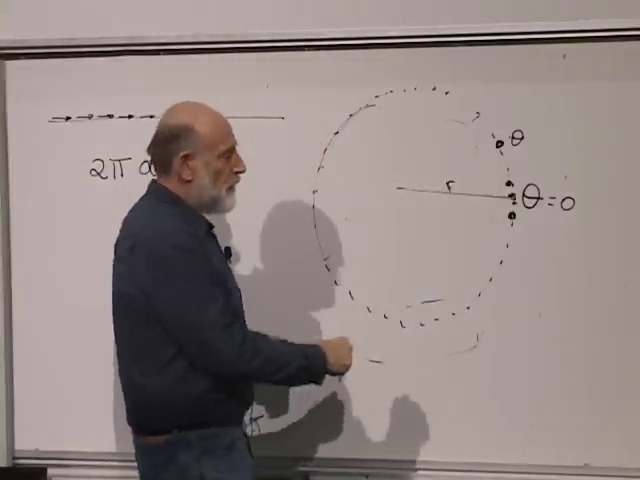
\includegraphics[width=0.82\textwidth]{lecture_01_figure_03.png}
\caption{Mô tả góc của một vũ trụ một chiều đóng, với tổng chu vi là \(2\pi a\).}
\end{figure}

Một quy ước thuận tiện là\footnote{Trong khoảng 01:26:40--01:29:20, ký hiệu tạm thời chuyển qua lại giữa việc lấy chính toàn bộ chu vi làm thừa số tỉ lệ và viết nó thành \(2\pi a\). Ở đây dùng quy ước sau, vì đó là quy ước được mang vào công thức độ dài cung.}
\begin{equation}
L=2\pi a,
\end{equation}
trong đó \(L\) là tổng chu vi.

Với một độ tách góc nhỏ \(\Delta\theta\), khoảng cách vật lý là
\begin{equation}
d=a\,\Delta\theta.
\end{equation}
Chuyển sang các vi phân cho
\begin{equation}
ds=a\,d\theta,
\end{equation}
và do đó
\begin{equation}
ds^2=a^2\,d\theta^2.
\end{equation}
Đây là metric cục bộ trên đường tròn.

Nếu \(a\) phụ thuộc vào thời gian, thì vũ trụ một chiều đóng sẽ giãn nở hoặc co lại. Với một cặp thiên hà cố định,
\begin{equation}
d(t)=a(t)\,\Delta\theta,
\end{equation}
nên
\begin{equation}
\dot d=\dot a\,\Delta\theta
      =\frac{\dot a}{a}\,d.
\end{equation}
Định luật Hubble cũng vẫn đúng ở đây, ít nhất đối với những cặp không cách nhau xa đến mức đường đi theo phía còn lại quanh đường tròn trở nên mơ hồ.

Metric không-thời gian khi đó là
\begin{equation}
d\tau^2=dt^2-a^2(t)\,d\theta^2.
\end{equation}
Nếu \(a\) là hằng số, thì hình ảnh không-thời gian là một hình trụ. Nếu \(a\propto t\), thì đó là một hình nón. Nếu \(a(t)\) biến thiên bất quy tắc hơn, thì hình ảnh sẽ giống một cái bình.

Nếu cho bức tranh chạy ngược theo thời gian, các thiên hà sẽ càng lúc càng gần nhau hơn. Nếu có \(360\) thiên hà quanh đường tròn, thì ở các thời điểm muộn chúng sẽ phân bố khá đều, ở thời điểm sớm hơn thì rất sít nhau, rồi còn sít hơn nữa. Cuối cùng chúng sẽ không còn là những thiên hà tách biệt nữa, và sớm hơn nữa thì thậm chí các nguyên tử cũng không còn tách biệt. Nhưng vẫn không có điểm đặc biệt nào trong không gian.

Đó là câu trả lời sáng sủa nhất cho câu hỏi Vụ Nổ Lớn đã xảy ra ở đâu trong mô hình này. Khi \(a(t)\to 0\), mọi khoảng tách \(a(t)\,\Delta\theta\) đều tiến về không. Toàn bộ vũ trụ co lại ở khắp nơi cùng một lúc. Các thiên hà không bay ra xa khỏi một vị trí đặc quyền nào đó trong một không gian bên ngoài. Chính hình học tự nó đang đổi thang. Theo nghĩa đó, câu trả lời là: ở khắp mọi nơi.

\begin{classroomqa}
\audiencequestion{Ông nói không-thời gian là cong. Nếu nó là một hình trụ thì nó có cong không?}\lecturetimestamp{01:38:04}
\lecturerresponse{Không. Nếu nó là một hình trụ thì nó sẽ không cong. Đó là trường hợp \(a\) không đổi theo thời gian. Nó chỉ trông cong vì được vẽ trong một không gian có số chiều cao hơn. Nếu cắt nó ra, có thể trải phẳng nó mà không cần kéo giãn.}
\end{classroomqa}

Từ đó cuộc thảo luận chuyển sang hình nón. Nếu \(a\propto t\), hình ảnh không-thời gian là một hình nón. Xa chóp của nó, hình nón cũng phẳng theo cùng nghĩa nội tại đó: có thể mở nó ra thành một mặt phẳng. Chóp thì khác. Đó là một kỳ dị hình nón.

Bước tiếp theo là hình học của vũ trụ hình cầu, rồi đến động lực học quyết định \(a(t)\) tăng lên hay co lại như thế nào.
